%\documentclass[c]{beamer}  % [t], [c], или [b] --- вертикальное выравнивание на слайдах (верх, центр, низ)
%\documentclass[handout]{beamer} % Раздаточный материал (на слайдах всё сразу)
\documentclass{beamer} % Соотношение сторон

%\usetheme{Berkeley} % Тема оформления
%\usetheme{Bergen}
\usetheme[progressbar = frametitle]{metropolis}
\setbeamertemplate{frame numbering}[fraction]
\useoutertheme{metropolis}
\useinnertheme{metropolis}
\usefonttheme{metropolis}
\usecolortheme{dolphin} % Цветовая схема
\setbeamercolor{background canvas}{bg=white}
%\useinnertheme{circles}
%\useinnertheme{rectangles}

%%% Работа с русским языком
\usepackage{cmap}					% поиск в PDF
\usepackage{mathtext} 				% русские буквы в формулах
\usepackage[T2A]{fontenc}			% кодировка
\usepackage[utf8]{inputenc}			% кодировка исходного текста
\usepackage[english,russian]{babel}	% локализация и переносы

%% Beamer по-русски
\newtheorem{rtheorem}{Теорема}
\newtheorem{rproof}{Доказательство}
\newtheorem{rexample}{Пример}

%%% Дополнительная работа с математикой
\usepackage{amsmath,amsfonts,amssymb,amsthm,mathtools} % AMS
\usepackage{icomma} % "Умная" запятая: $0,2$ --- число, $0, 2$ --- перечисление

%% Номера формул
%\mathtoolsset{showonlyrefs=true} % Показывать номера только у тех формул, на которые есть \eqref{} в тексте.
%\usepackage{leqno} % Нумерация формул слева

%% Свои команды
\DeclareMathOperator{\sgn}{\mathop{sgn}}

%% Перенос знаков в формулах (по Львовскому)
\newcommand*{\hm}[1]{#1\nobreak\discretionary{}
	{\hbox{$\mathsurround=0pt #1$}}{}}

%%% Работа с картинками
\usepackage{graphicx}  % Для вставки рисунков
\setlength\fboxsep{3pt} % Отступ рамки \fbox{} от рисунка
\setlength\fboxrule{1pt} % Толщина линий рамки \fbox{}
\usepackage{wrapfig} % Обтекание рисунков текстом

%%% Работа с таблицами
\usepackage{array,tabularx,tabulary,booktabs} % Дополнительная работа с таблицами
\usepackage{longtable}  % Длинные таблицы
\usepackage{multirow} % Слияние строк в таблице

%%% Программирование
\usepackage{etoolbox} % логические операторы

%%% Другие пакеты
\usepackage{lastpage} % Узнать, сколько всего страниц в документе.
\usepackage{soul} % Модификаторы начертания
\usepackage{csquotes} % Еще инструменты для ссылок
%\usepackage[style=authoryear,maxcitenames=2,backend=biber,sorting=nty]{biblatex}
\usepackage{multicol} % Несколько колонок

%%% Картинки
\usepackage{tikz} % Работа с графикой
\usepackage{pgfplots}
\usepackage{pgfplotstable}
\usepackage{caption}
\usepackage{subcaption}
\usepackage{diagbox}

\usepackage{dsfont}
\newcommand{\R}{\mathbb{R}}
\newcommand{\norm}[1]{\lVert #1 \rVert_2}

\title{Собеседование на специализацию <<Интеллектуальный анализ данных>>}
\author{Киселев Никита Б05-002}
\date{\today}
\institute[Московский физико-технический институт]{Московский физико-технический институт \\ (национальный исследовательский университет)}

\setbeamercovered{transparent = 15}
\graphicspath{{../}}

\begin{document}
\metroset{block = fill}
	
	\begin{frame}
		\maketitle
	\end{frame}

	\begin{frame}{Тестовая задача}
        \textbf{Задача 21}

        Предсказание площади лесных пожаров. На основе погодных измерений необходимо 
        предсказать объем выгоревших лесных массивов на севере Португалии. Выборка 
        состоит из 13 признаков и 517 объектов. Для решения задачи предлагается 
        использовать метод наименьших квадратов с регуляризацией. Нарисовать график 
        весов признаков и общей ошибки на кросс-валидации при изменении параметра 
        регуляризации. Какие признаки наиболее важны для нашей задачи? Что изменится, 
        если предварительно все признаки стандартизовать?
    \end{frame}
	
    \begin{frame}{Распределение ответов}
        \begin{figure}[h!]
            \centering
            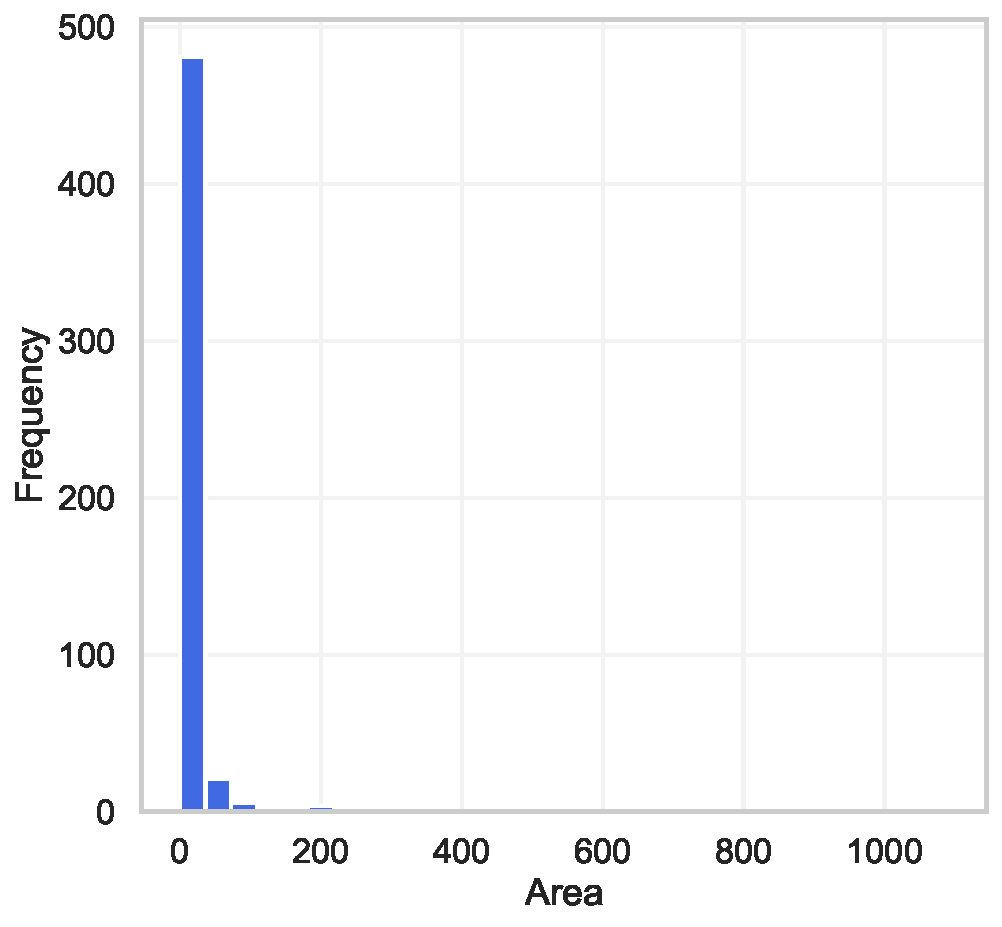
\includegraphics[scale = 0.5]{area_distribution.pdf}
        \end{figure}
    \end{frame}

    \begin{frame}{Распределение номинальных признаков}
        \begin{figure}[h!]
            \centering
            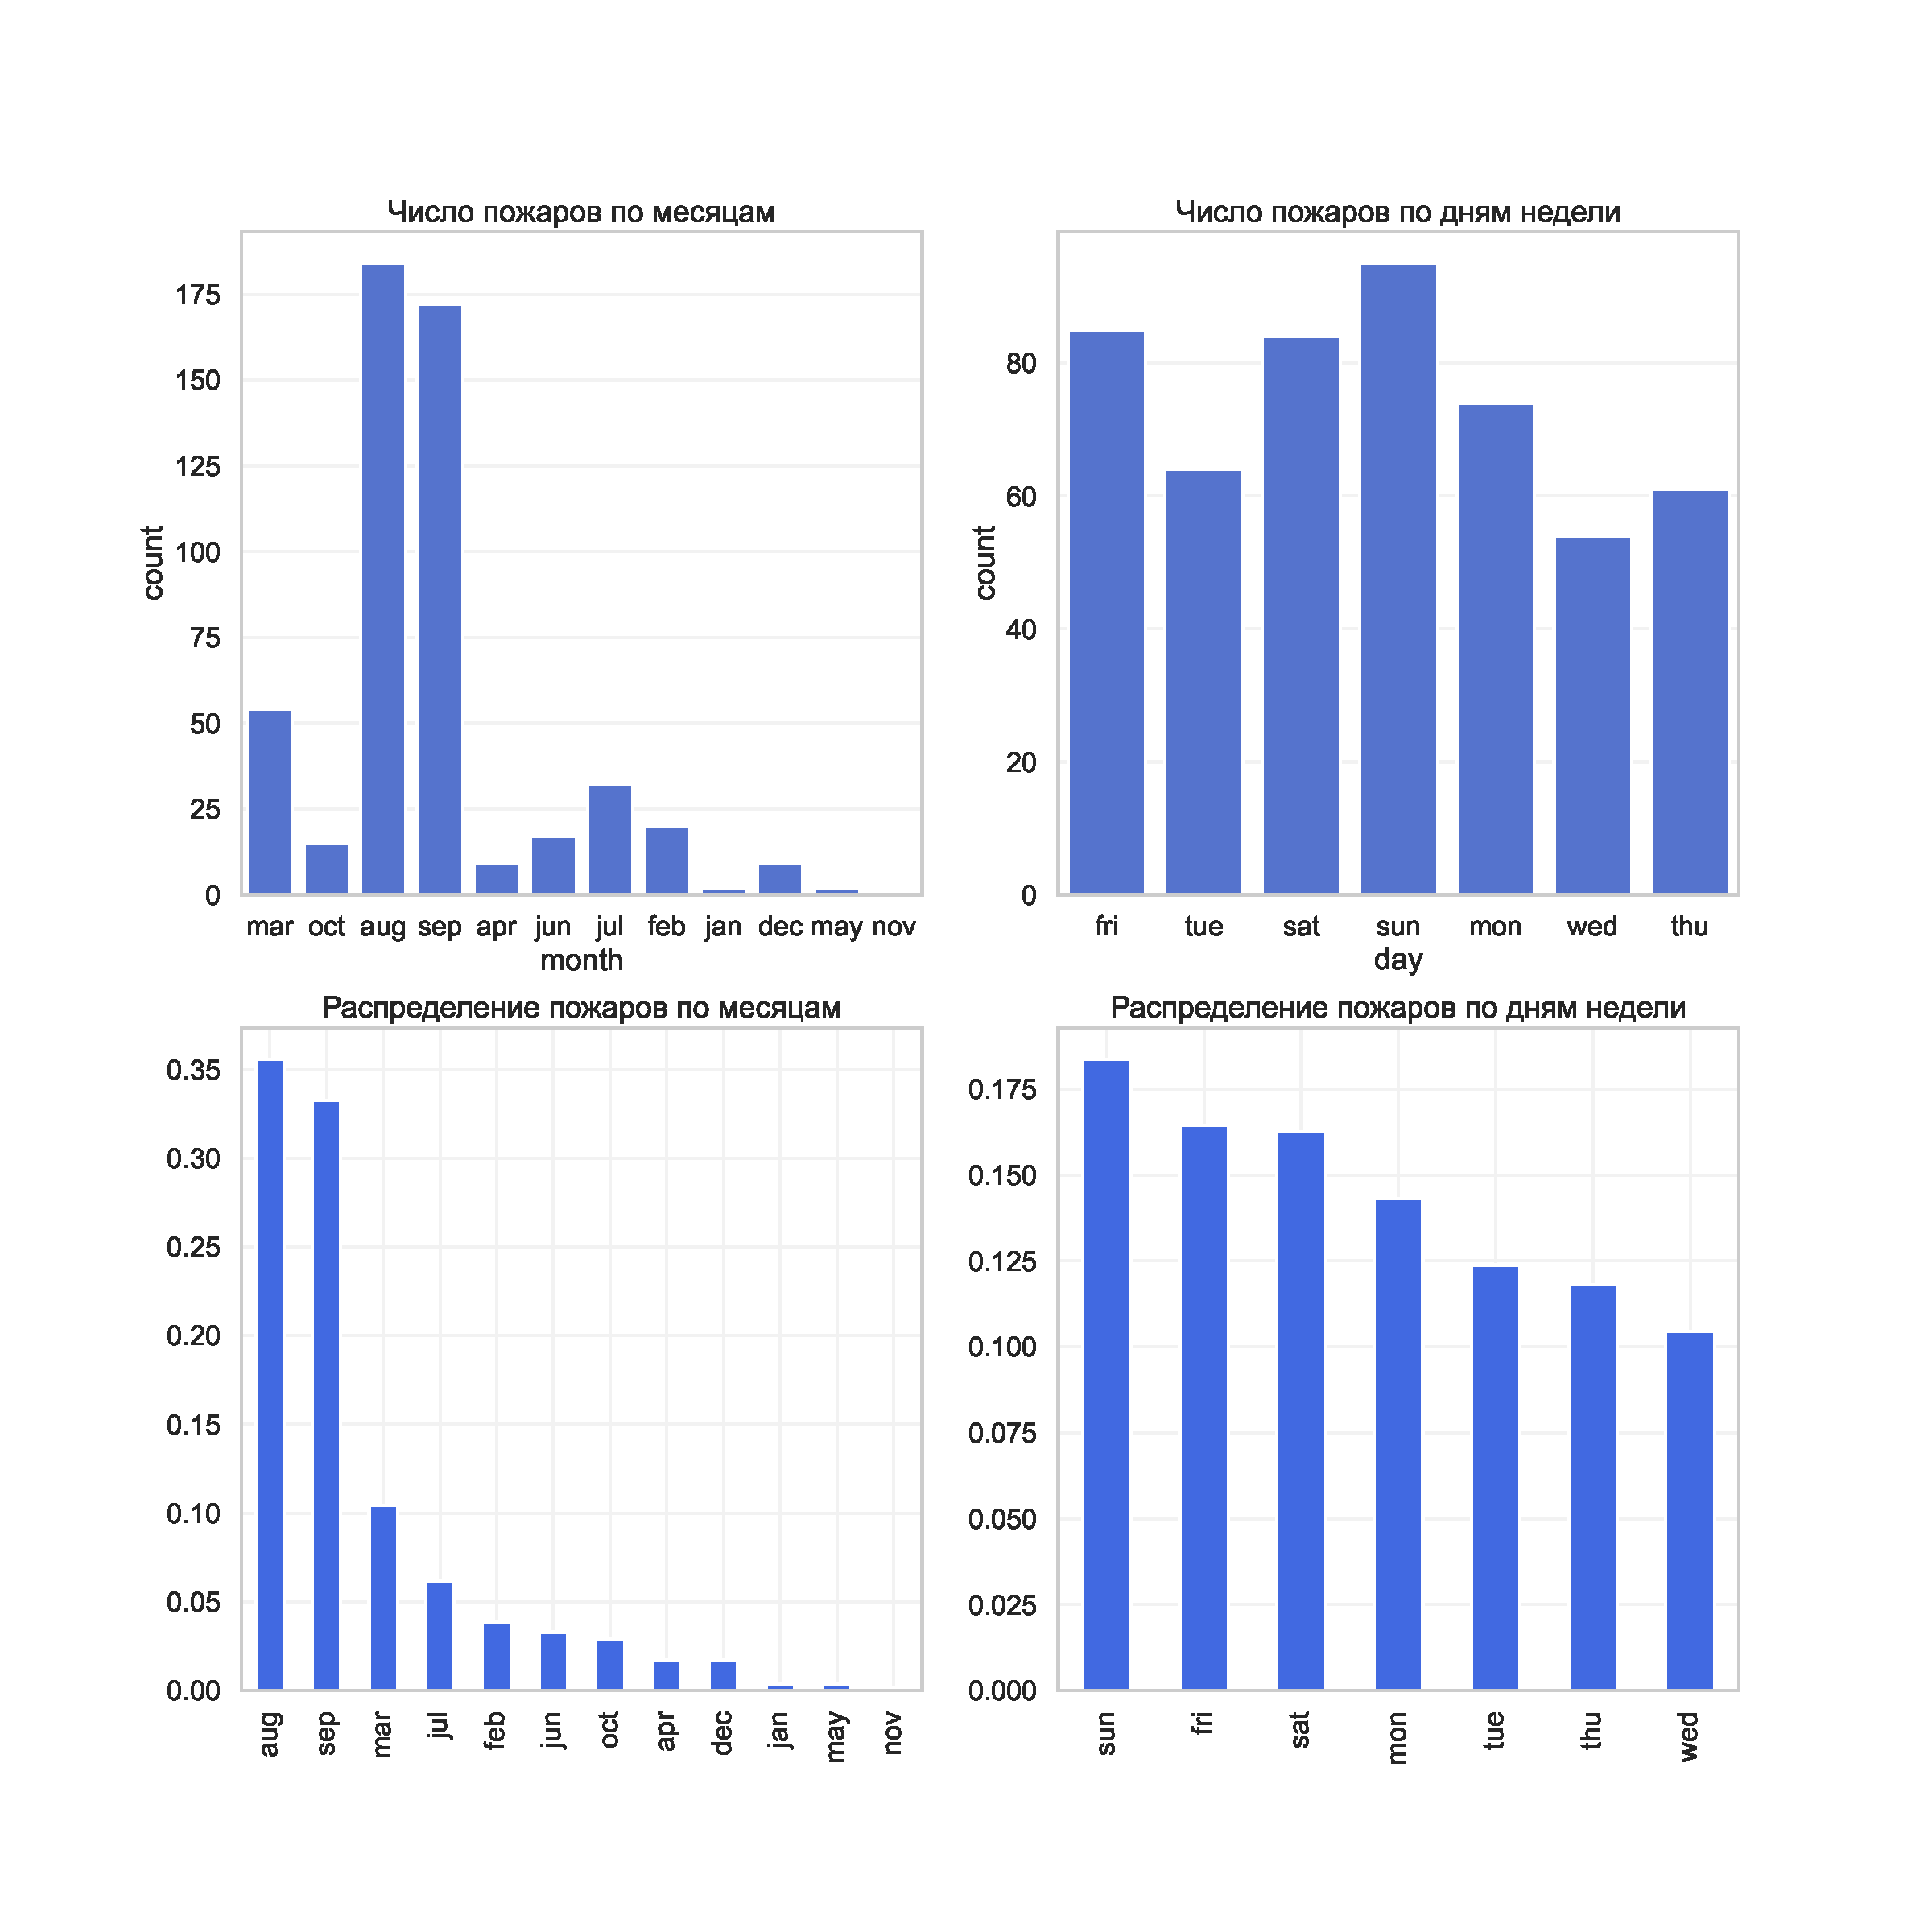
\includegraphics[scale = 0.2]{cat_features.pdf}
        \end{figure}
    \end{frame}

    \begin{frame}{Корреляция количественных признаков}
        \begin{figure}[h!]
            \centering
            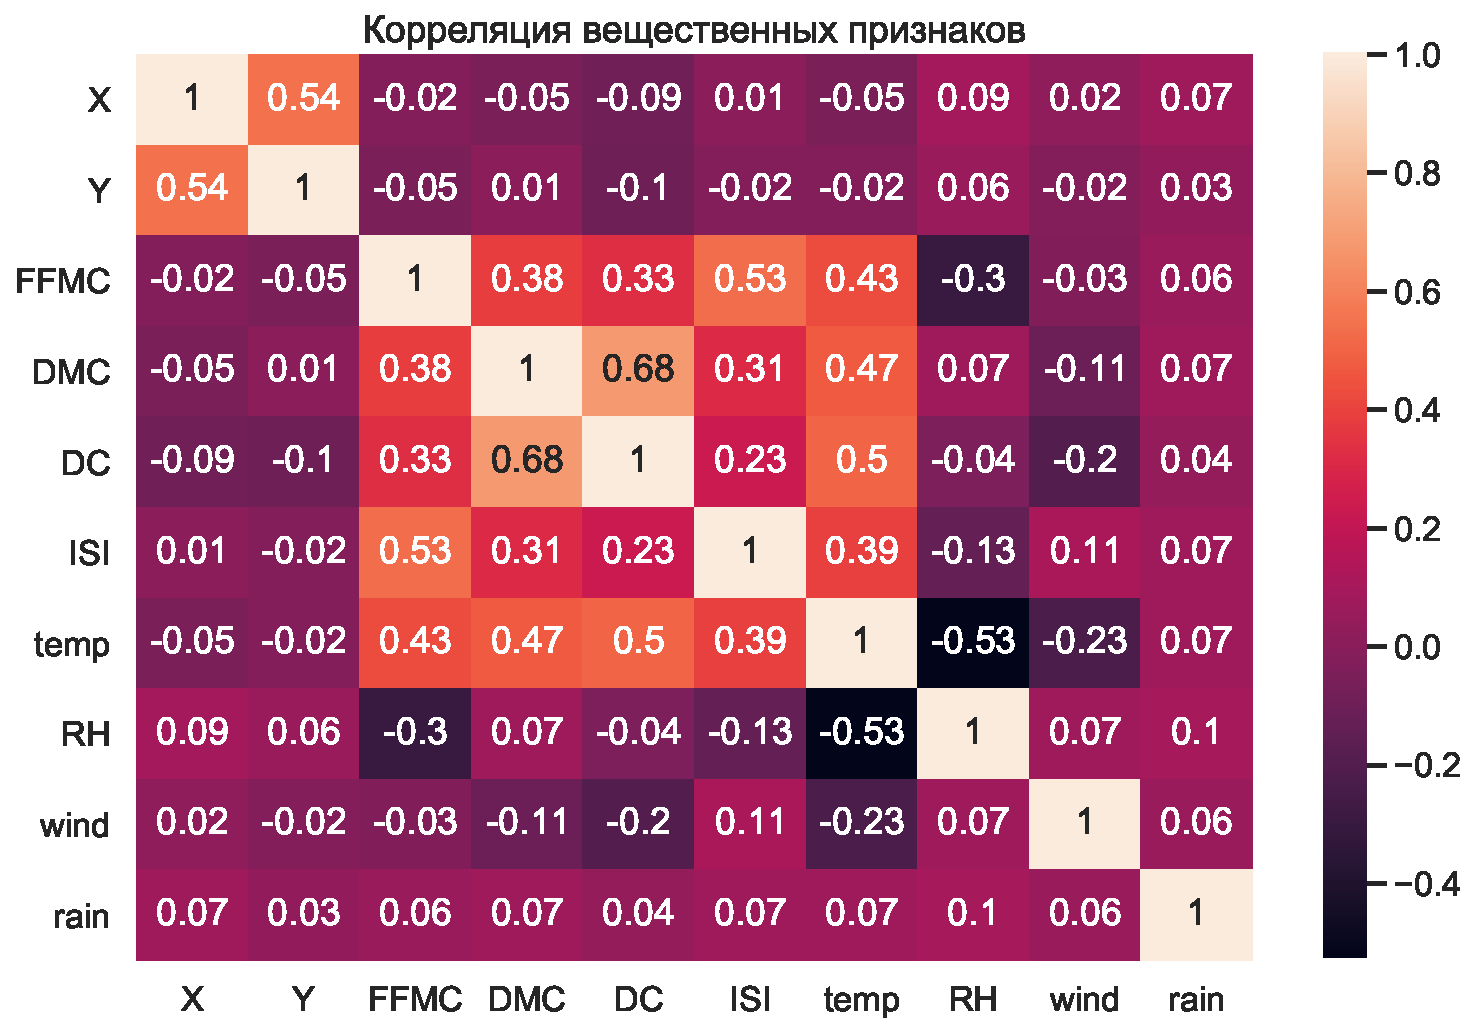
\includegraphics[scale = 0.35]{num_features_corr.pdf}
        \end{figure}
    \end{frame}

    \begin{frame}{Линейная регрессия}
        \begin{itemize}
            \item Множество объектов $\mathds{X} = \R^n$
            \item Объекту $\mathbf{x} \in \mathds{X}$ соответствует признаковое описание $\mathbf{x} = (f_1(x), \ldots, f_n(x))$,
            где $f_j: \mathbf{X} \to D_j$ 
            \item Множество ответов $\mathds{Y} = \R$
            \item Выборка $\mathds{D} = \{ (\mathbf{x}_i, y_i) \ | \ \mathbf{x}_i \in \mathds{X}, y_i \in \mathds{Y}, i = 1, \ldots, m \}$
            \item Матрица объекты-признаки $X = (\mathbf{x}_1, \ldots, \mathbf{x}_m)^T$, вектор ответов $\mathbf{y} \in \R^m$
            \item Вектор параметров модели $\mathbf{w} = (w_1, \ldots, w_n)^T$
            \item Ставится задача минимизации ошибки алгоритма $Q(w, X) = \lVert X \mathbf{w} - y \rVert_2^2 \to \min\limits_{\mathbf{w}}$
        \end{itemize}
    \end{frame}

    \begin{frame}{Метод наименьших квадратов}
        \[ Q(\mathbf{w}, X) = \lVert X \mathbf{w} - y \rVert_2^2 = (X \mathbf{w} - y)^T (X \mathbf{w} - y) \to \min\limits_{\mathbf{w}} \]

        Приравняем к нулю производную по вектору $\mathbf{w}$:
        \begin{multline*}
            \nabla_{\mathbf{w}} Q(\mathbf{w}, X) = \nabla_{\mathbf{w}}(-y^T X \mathbf{w} + \mathbf{w}^T X^T X \mathbf{w} + y^T y - \mathbf{w}^T X^T y) = \\ 
            = - X^T y + (X^T X + X^T X) \mathbf{w} + 0 - X^T y = 0
        \end{multline*}
        \[ X^T X \mathbf{w} = X^T y \]
        \[ \fbox{$\mathbf{w}^* = (X^T X)^{-1} X^T y$} \]

    \end{frame}

    \begin{frame}{$L_2$ регуляризация}
        Могут возникнуть проблемы мультиколлинеарности в случае, если матрица $X^T X$ плохо обусловлена.
        Один из способов решения~--- добавление к этой матрице диагональной:
        \[ \fbox{$\mathbf{w}^* = (X^T X + \alpha E_n)^{-1} X^T y$} \]
        При этом значении вектора $w$ достигается минимум функционала ошибки
        \[ Q(\mathbf{w}, X, \alpha) = \norm{X \mathbf{w} - y}^2 + \alpha \lVert \mathbf{w} \rVert_2^2 \]
    \end{frame}

    \begin{frame}{Изменение параметра $\alpha$}
        \begin{figure}
            \centering
            \begin{subfigure}[b]{0.475\textwidth}
                \centering
                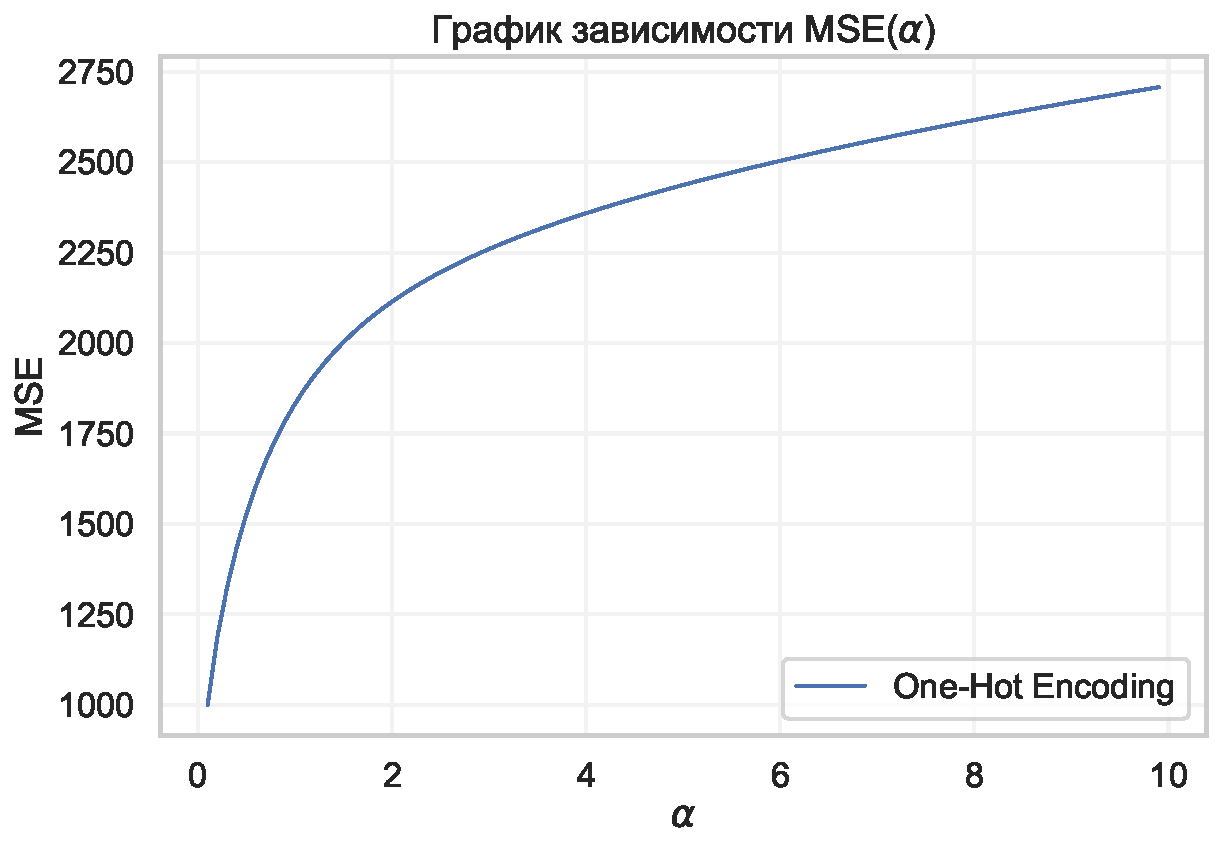
\includegraphics[width=\textwidth]{MSE_plot_oh.pdf}
            \end{subfigure}
            \hfill
            \begin{subfigure}[b]{0.475\textwidth}  
                \centering 
                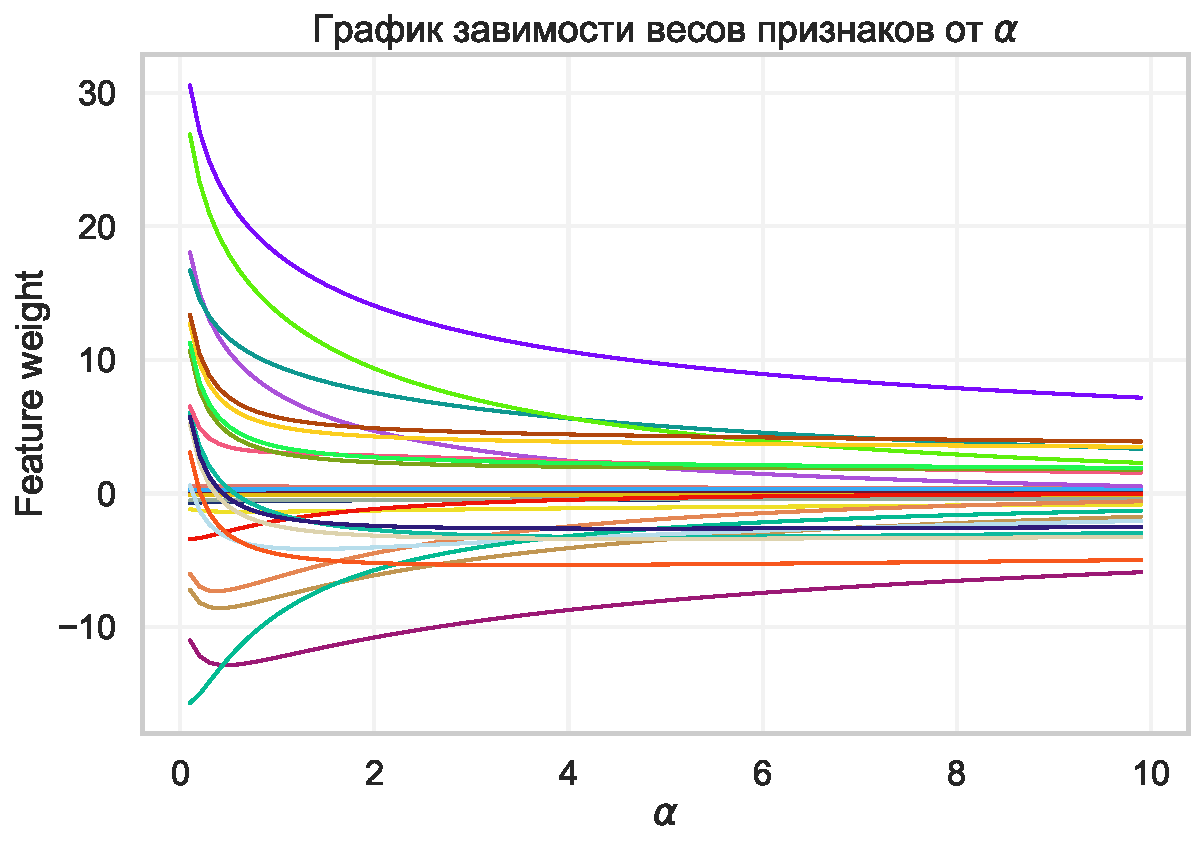
\includegraphics[width=\textwidth]{feature_plot_oh.pdf}
            \end{subfigure}
            \begin{subfigure}[b]{0.475\textwidth}   
                \centering 
                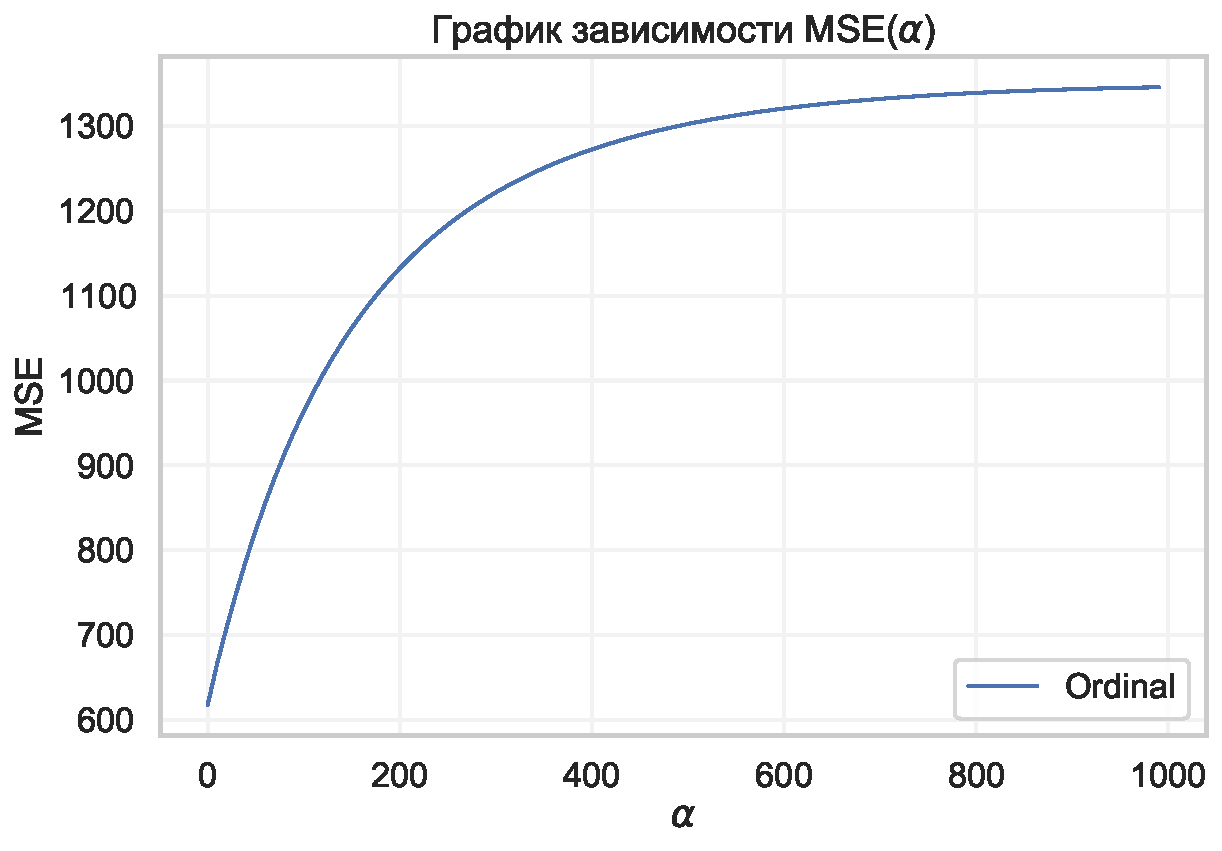
\includegraphics[width=\textwidth]{MSE_plot.pdf}
            \end{subfigure}
            \hfill
            \begin{subfigure}[b]{0.475\textwidth}   
                \centering 
                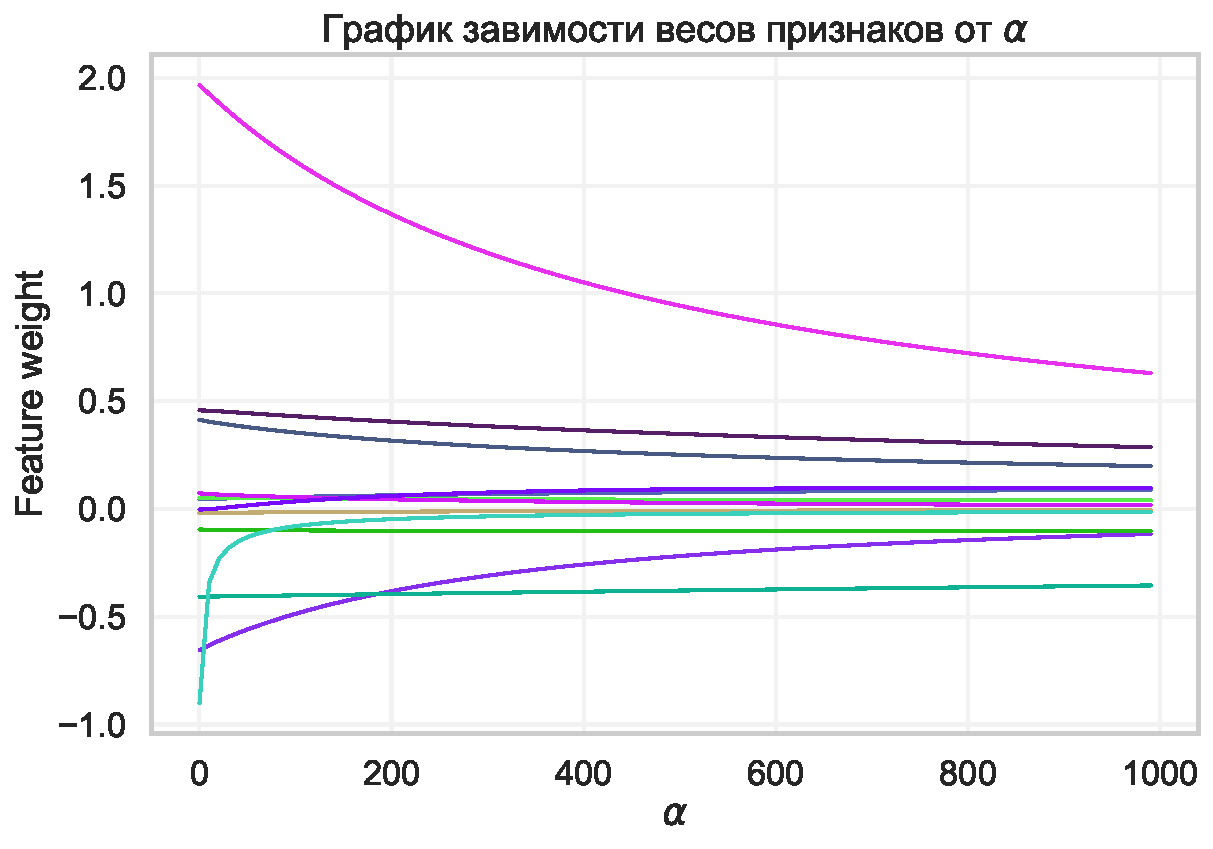
\includegraphics[width=\textwidth]{feature_plot.pdf}
            \end{subfigure} 
        \end{figure}
    \end{frame}

    \begin{frame}{Стандартизация}
        При стандартизации происходит преобразование признаков:
        \[ \hat{f}_j(\mathbf{x}_i) = \dfrac{f_j(\mathbf{x}_i) - \bar{f}_j}{S_j}, \]
        где 
        \[ \bar{f}_j = \dfrac{1}{m} \sum\limits_{i = 1}^m f_j(\mathbf{x}_i) \text{~--- выборочное среднее}, \]
        \[ S_j = \sqrt{\dfrac{1}{m} \sum\limits_{i=1}^m (f_j(\mathbf{x}_i) - \bar{f}_j)^2} \text{~--- среднеквадратичное отклонение}. \]
    \end{frame}

    \begin{frame}{Изменение параметра $\alpha$ при стандартизации}
        \begin{figure}
            \centering
            \begin{subfigure}[b]{0.475\textwidth}
                \centering
                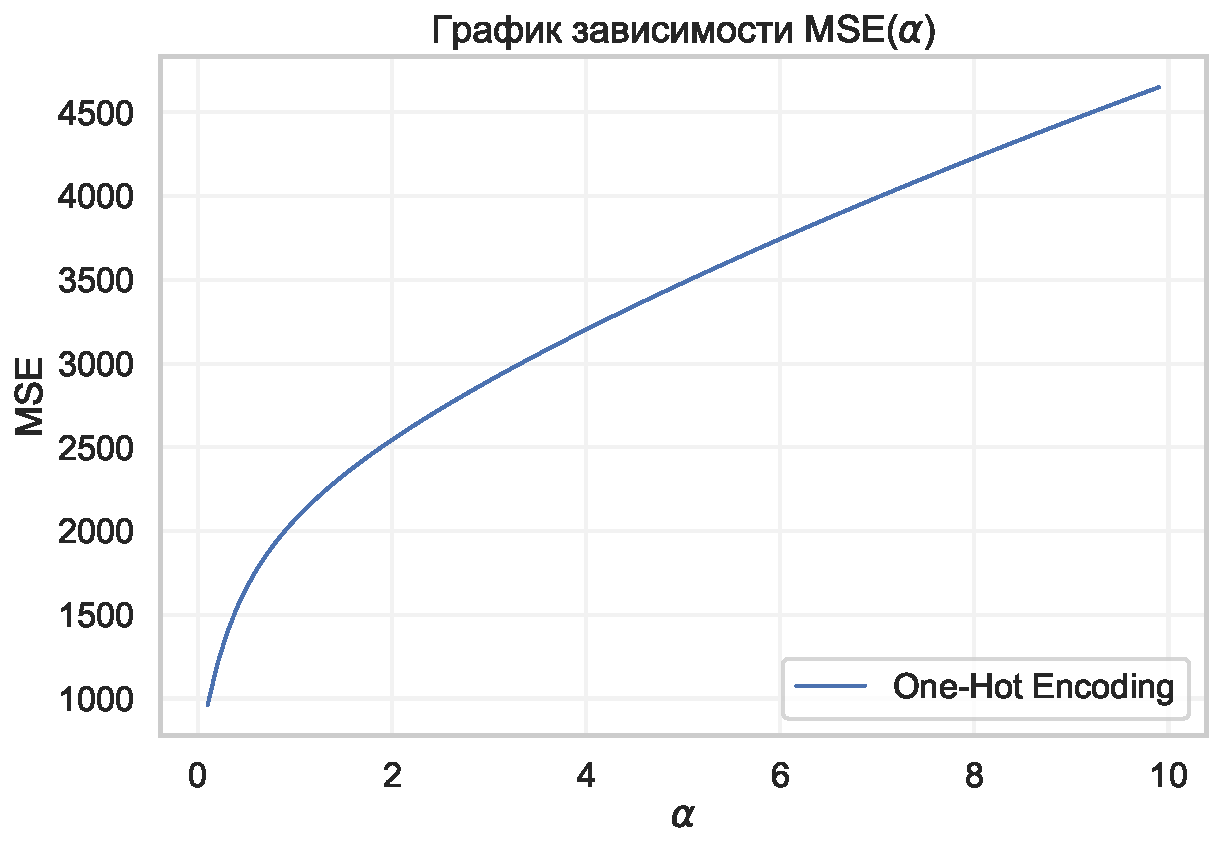
\includegraphics[width=\textwidth]{MSE_plot_oh_scaled.pdf}
            \end{subfigure}
            \hfill
            \begin{subfigure}[b]{0.475\textwidth}  
                \centering 
                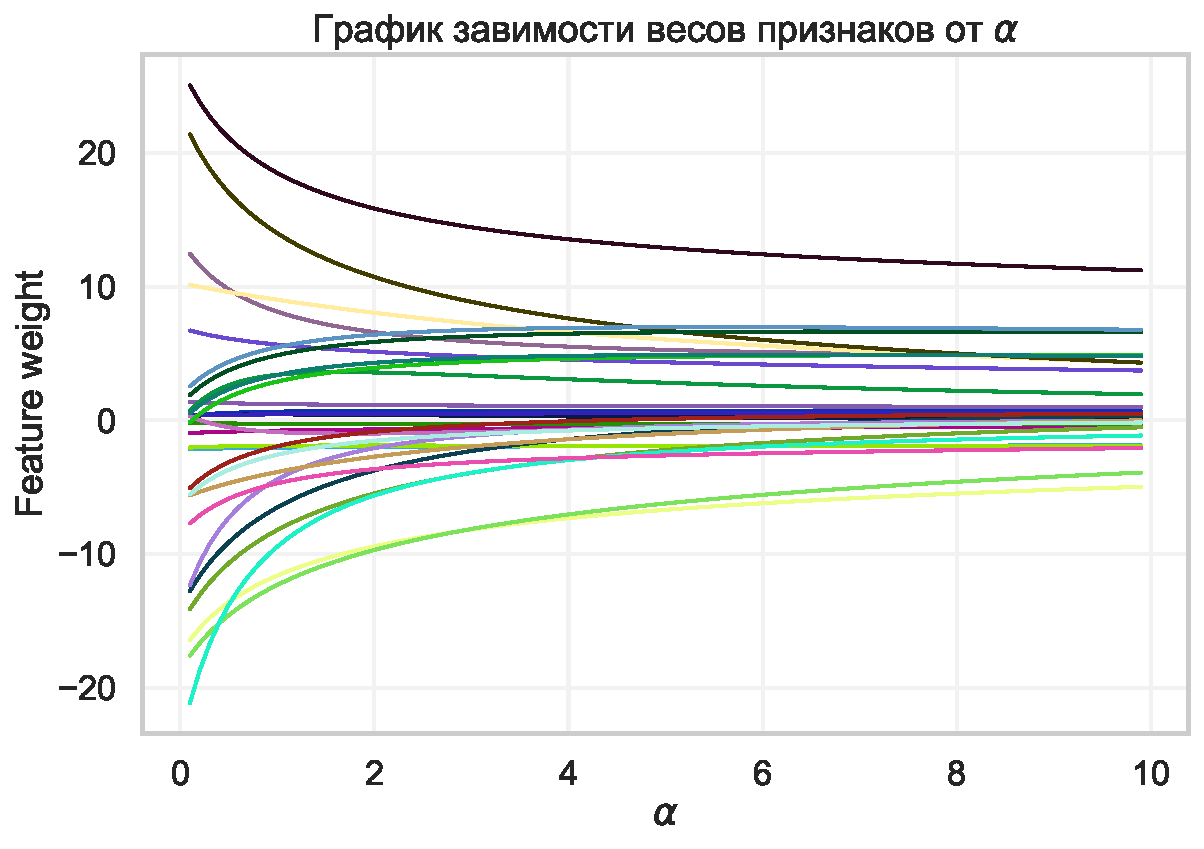
\includegraphics[width=\textwidth]{feature_plot_oh_scaled.pdf}
            \end{subfigure}
            \begin{subfigure}[b]{0.475\textwidth}   
                \centering 
                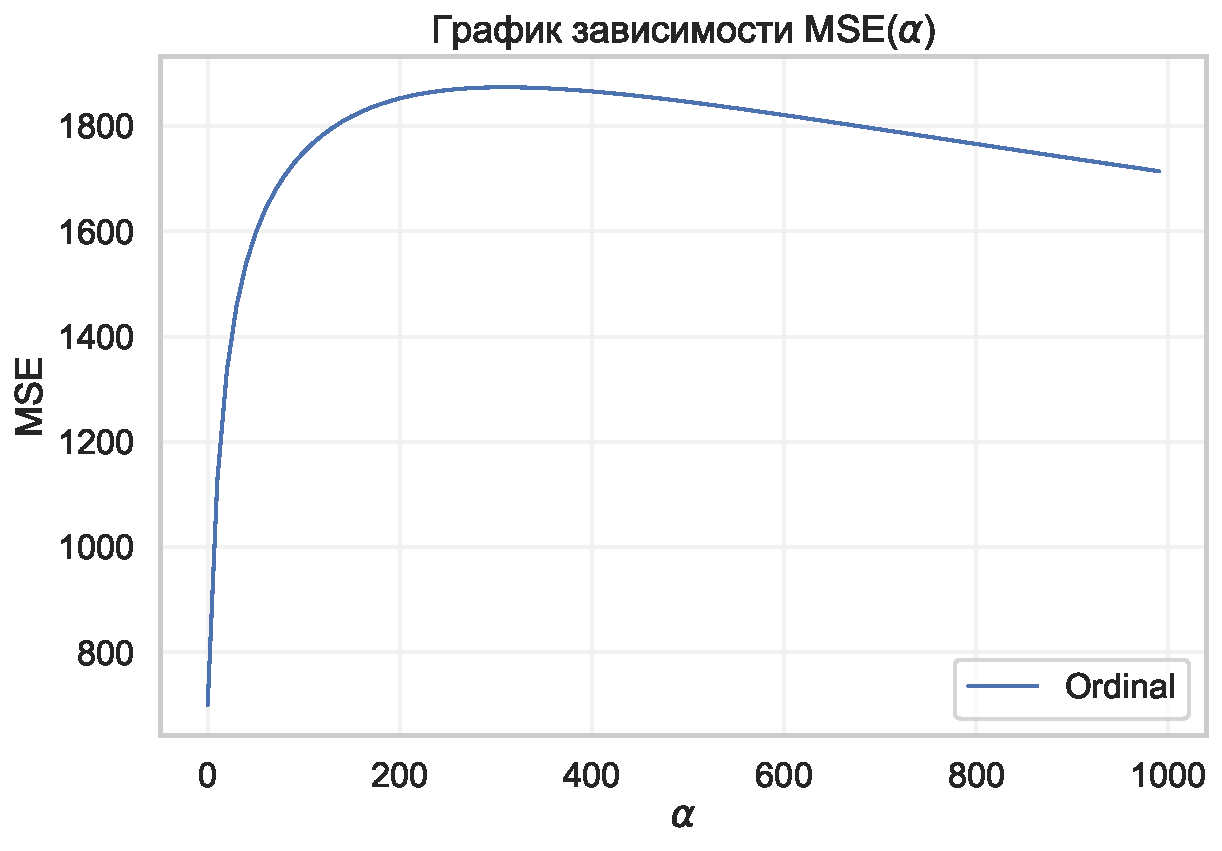
\includegraphics[width=\textwidth]{MSE_plot_scaled.pdf}
            \end{subfigure}
            \hfill
            \begin{subfigure}[b]{0.475\textwidth}   
                \centering 
                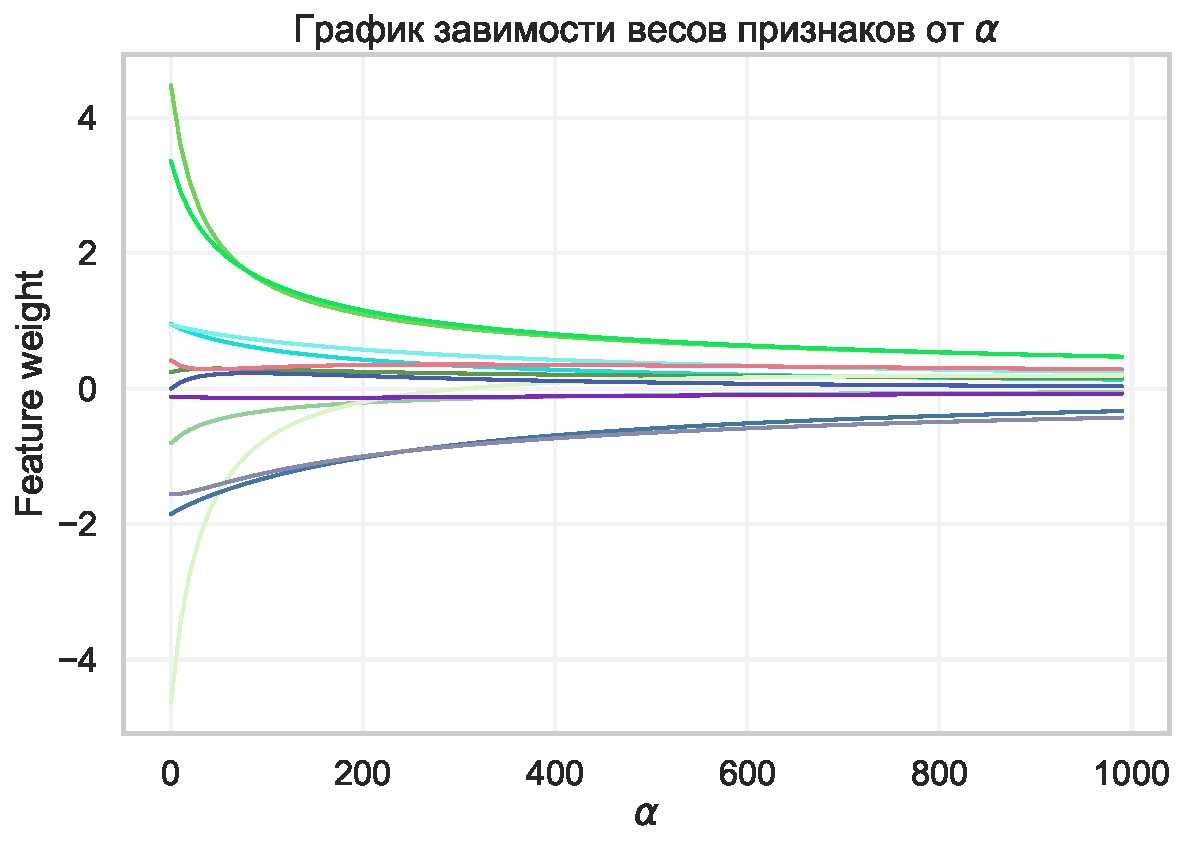
\includegraphics[width=\textwidth]{feature_plot_scaled.pdf}
            \end{subfigure} 
        \end{figure}
    \end{frame}

    \begin{frame}{Отбор признаков}
        \begin{figure}
            \centering
            \begin{subfigure}[b]{0.475\textwidth}
                \centering
                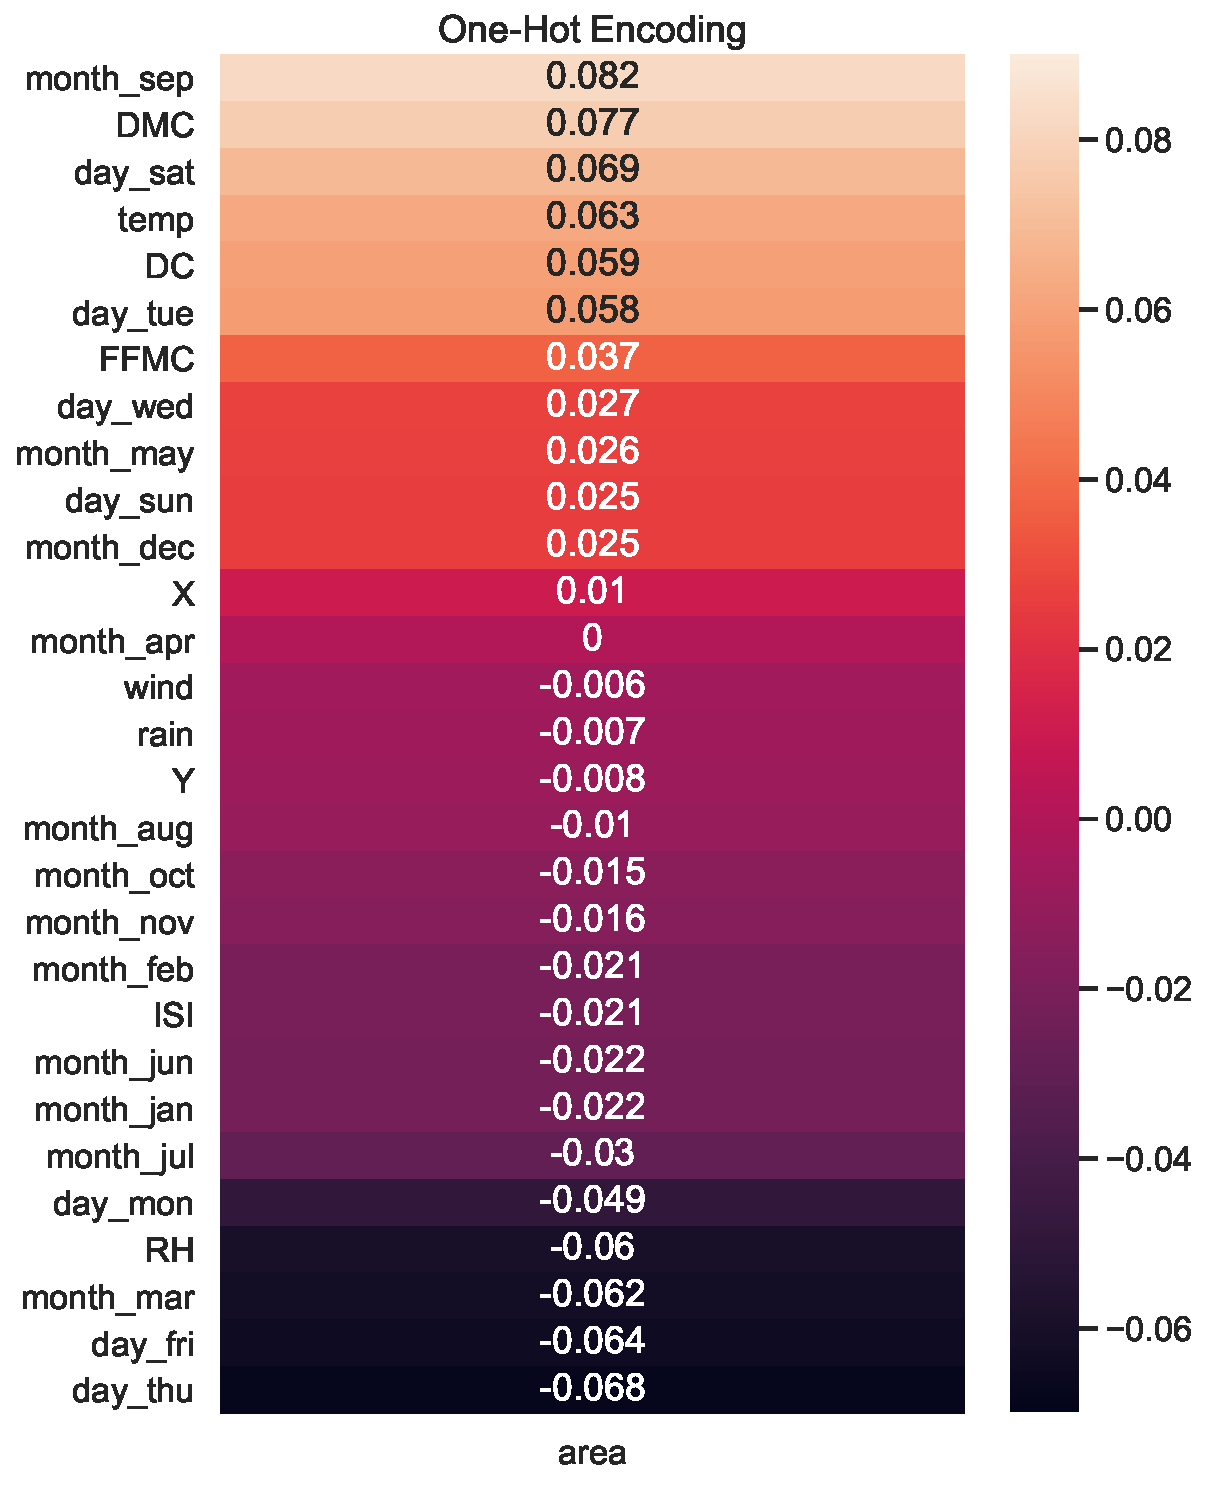
\includegraphics[width=\textwidth]{features_corr_oh.pdf}
            \end{subfigure}
            \hfill
            \begin{subfigure}[b]{0.475\textwidth}  
                \centering 
                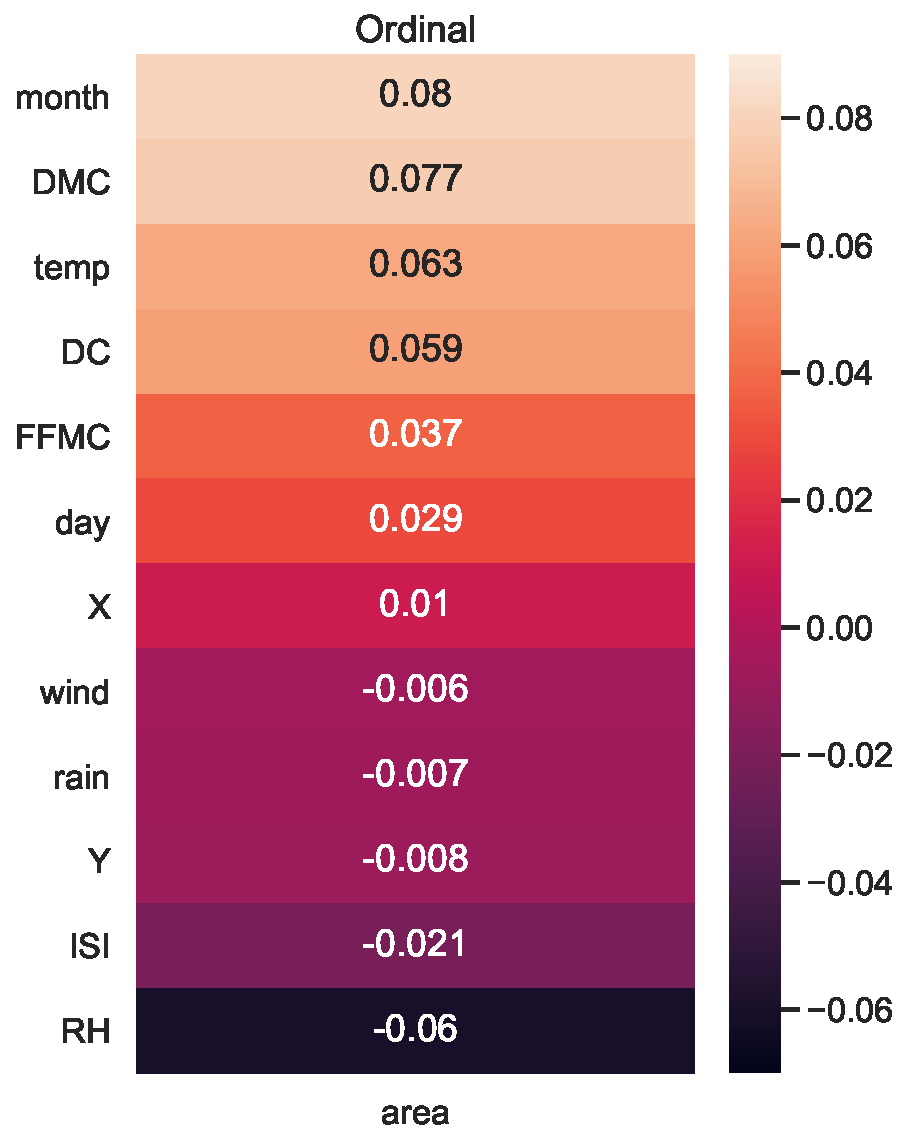
\includegraphics[width=\textwidth]{features_corr.pdf}
            \end{subfigure}
        \end{figure}
    \end{frame}

    \begin{frame}{Преобразования признаков и ответов}
        \begin{enumerate}
            \item rain~--- номинальный
            \item FFMC $\geq$ 75
            \item ISI $\to \ln(ISI)$
            \item area $\to \ln(1 + area)$
        \end{enumerate}
    \end{frame}

    \begin{frame}{Взаимосвязь новых признаков и ответов}
        \begin{figure}
            \centering
            \begin{subfigure}[b]{0.475\textwidth}
                \centering
                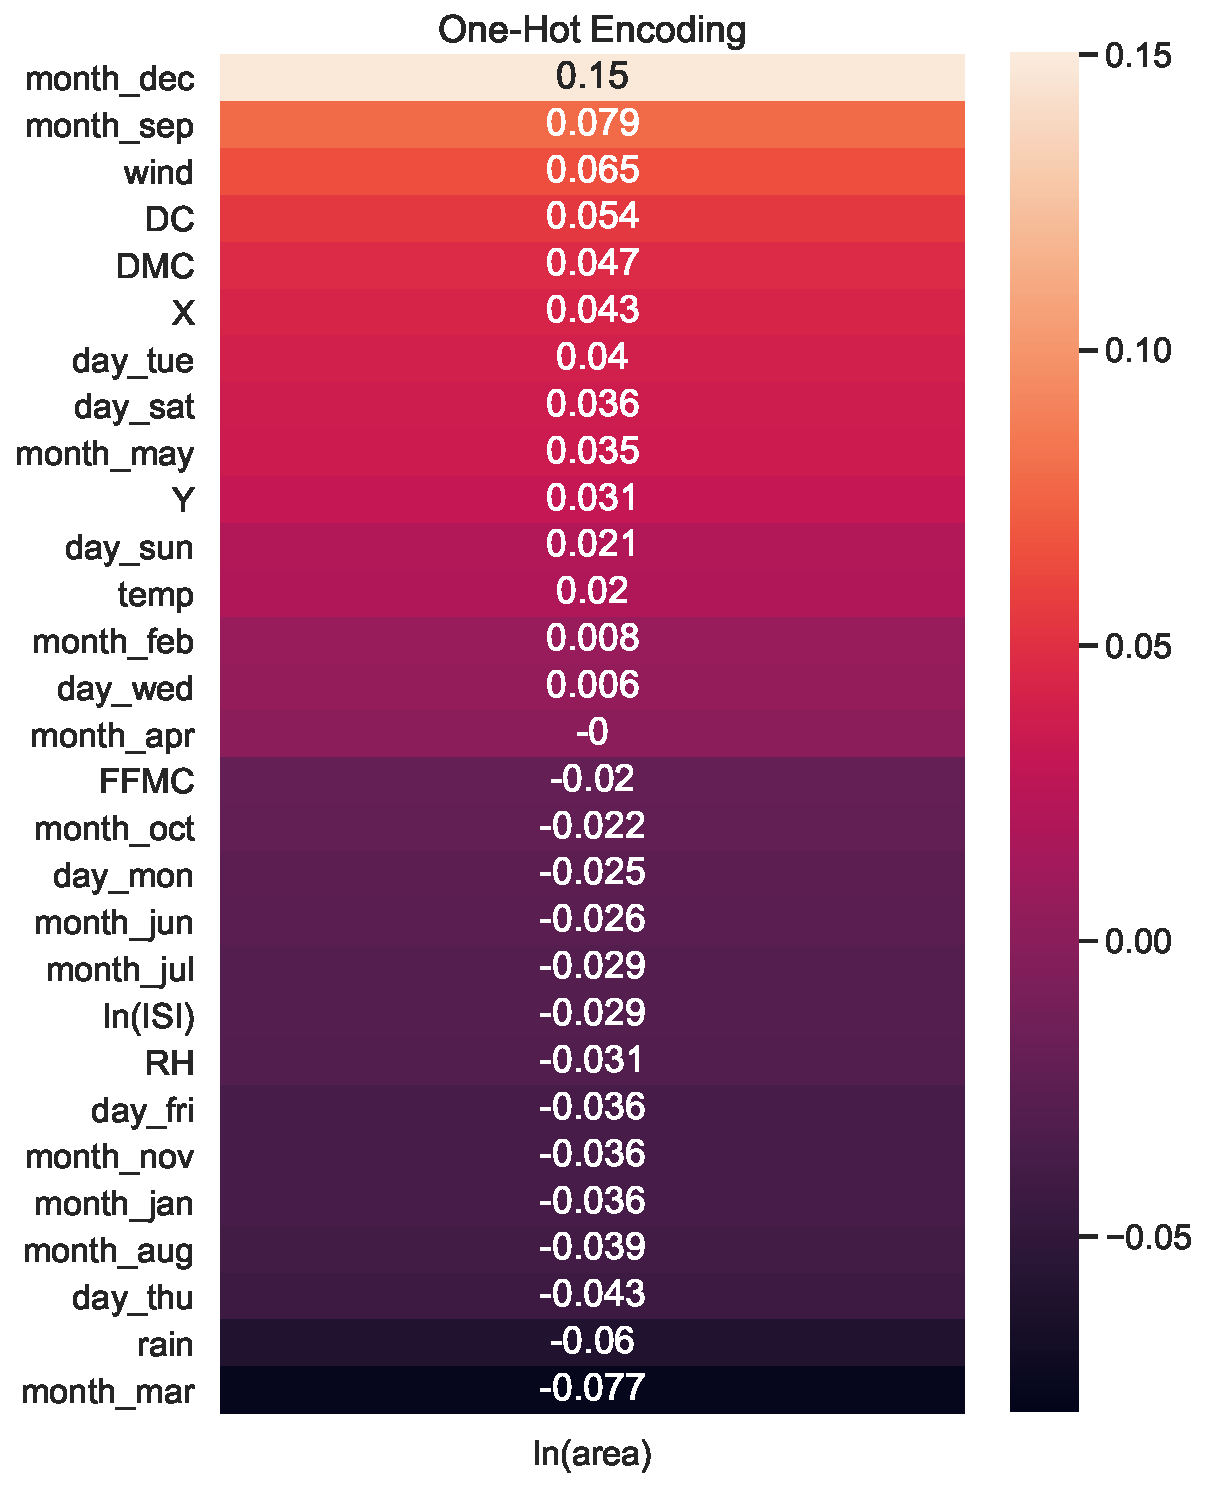
\includegraphics[width=\textwidth]{features_corr_oh_1.pdf}
            \end{subfigure}
            \hfill
            \begin{subfigure}[b]{0.475\textwidth}  
                \centering 
                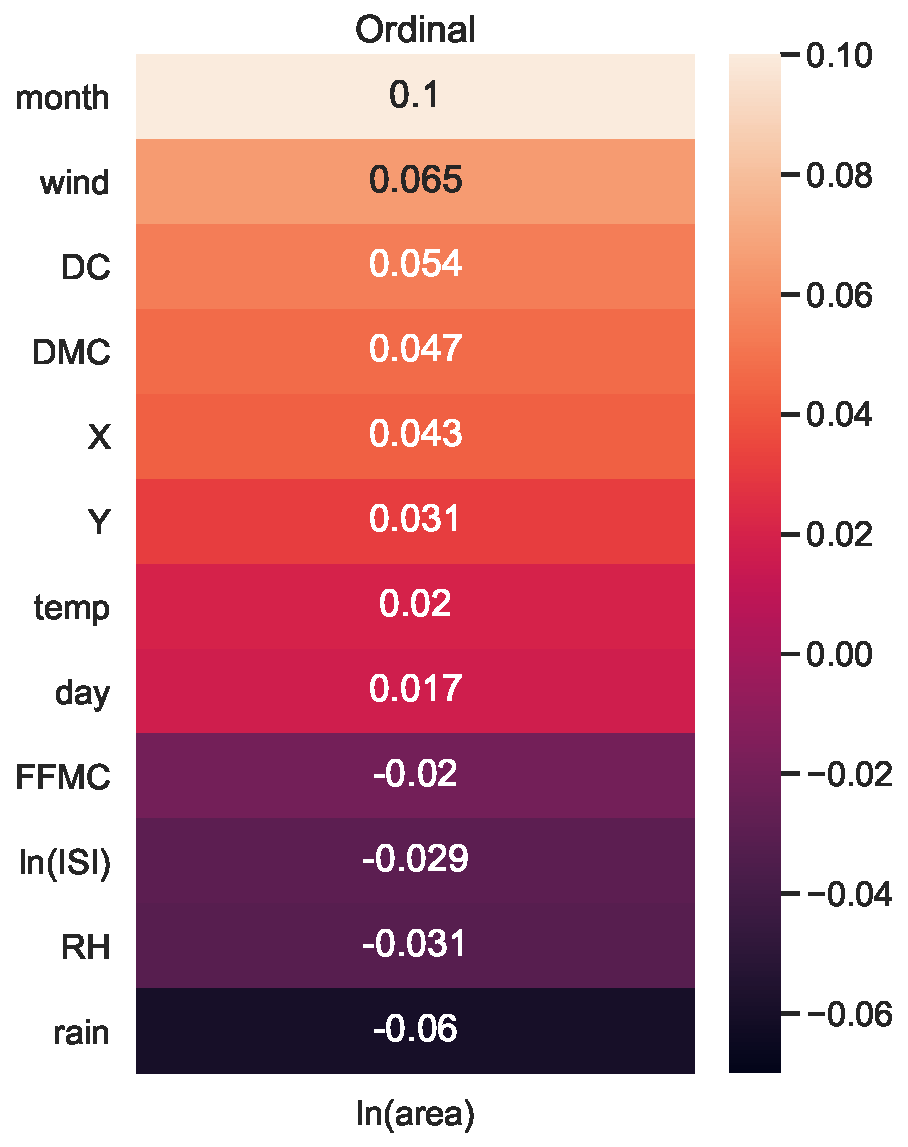
\includegraphics[width=\textwidth]{features_corr_1.pdf}
            \end{subfigure}
        \end{figure}
    \end{frame}

    \begin{frame}{Изменение параметра $\alpha$}
        \begin{figure}
            \centering
            \begin{subfigure}[b]{0.475\textwidth}
                \centering
                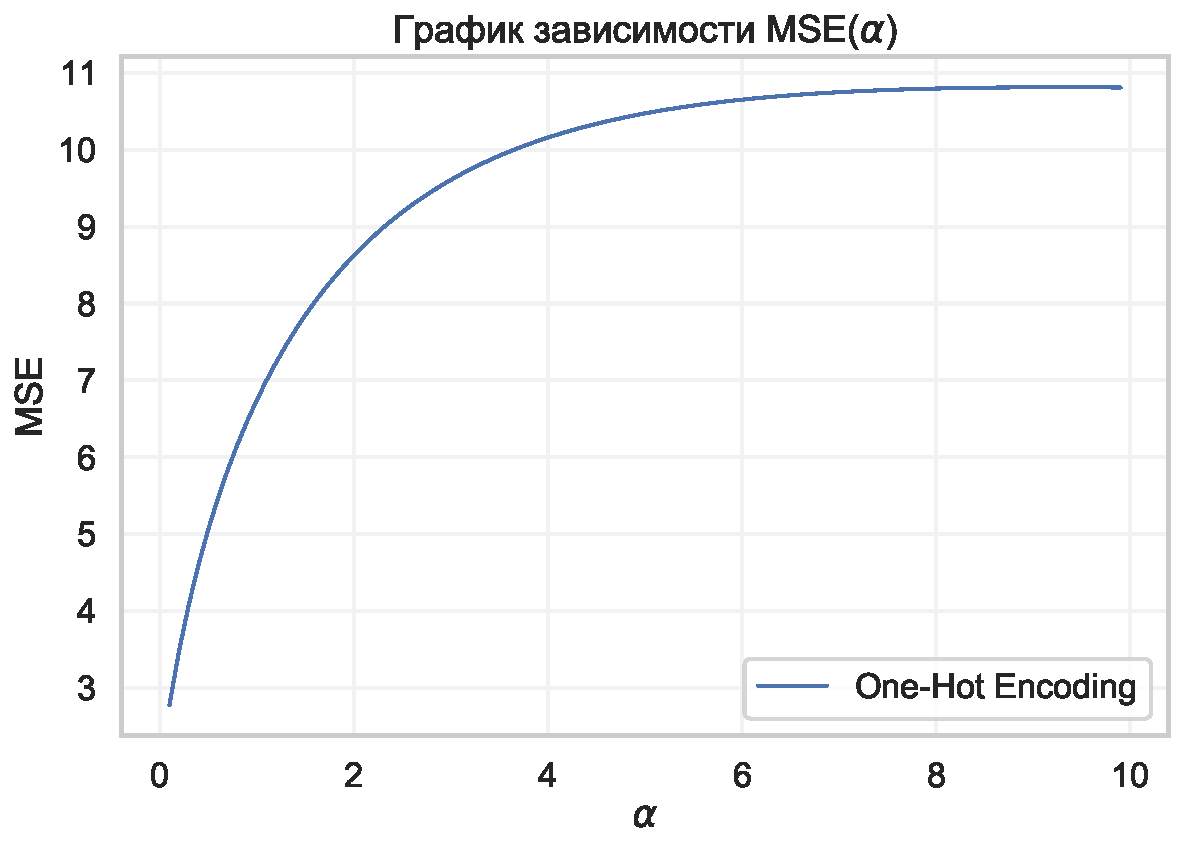
\includegraphics[width=\textwidth]{MSE_plot_oh_1.pdf}
            \end{subfigure}
            \hfill
            \begin{subfigure}[b]{0.475\textwidth}  
                \centering 
                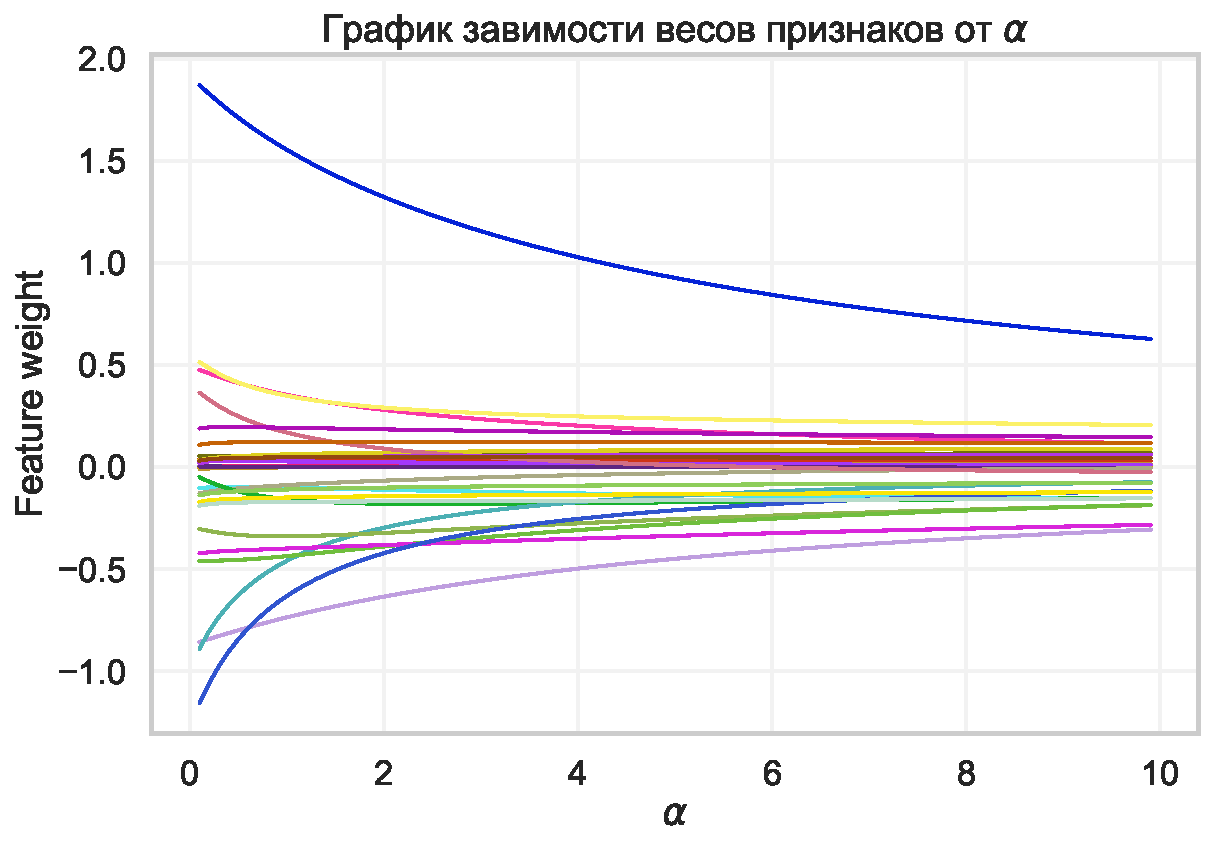
\includegraphics[width=\textwidth]{feature_plot_oh_1.pdf}
            \end{subfigure}
            \begin{subfigure}[b]{0.475\textwidth}   
                \centering 
                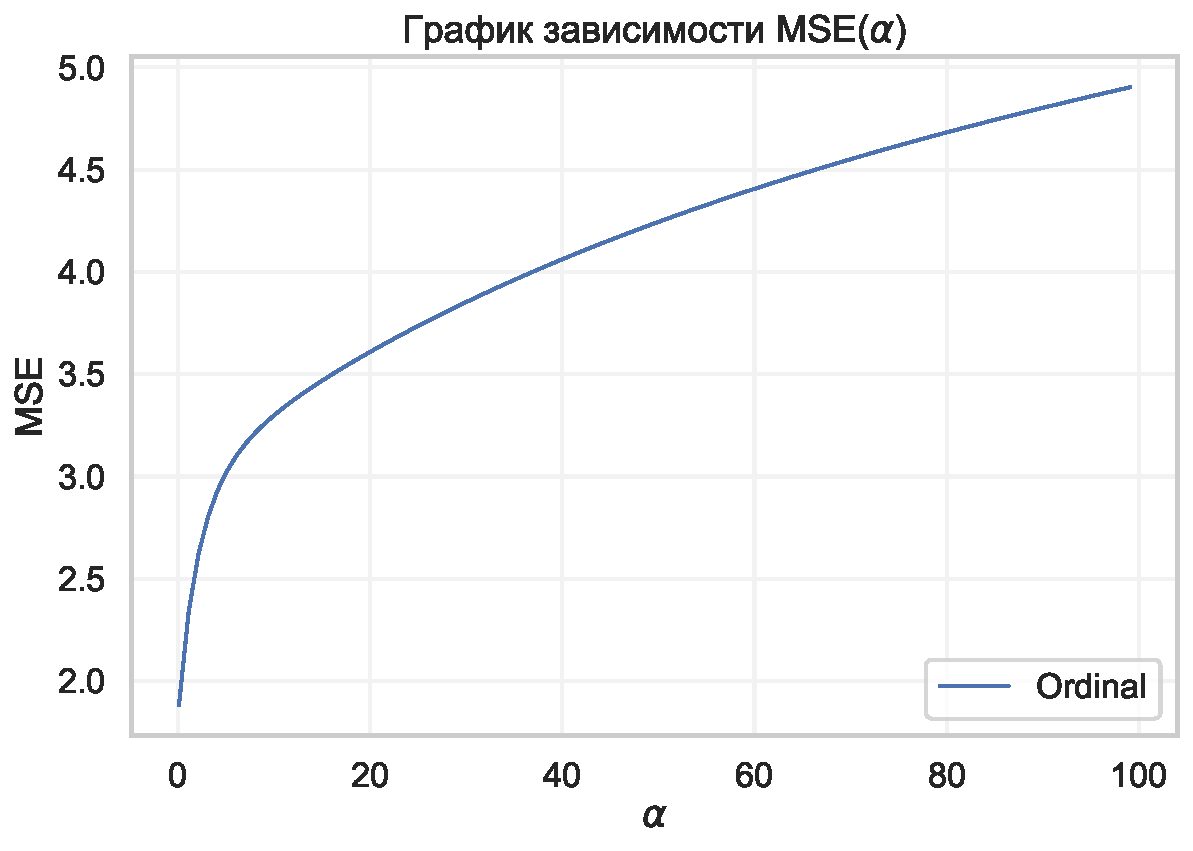
\includegraphics[width=\textwidth]{MSE_plot_1.pdf}
            \end{subfigure}
            \hfill
            \begin{subfigure}[b]{0.475\textwidth}   
                \centering 
                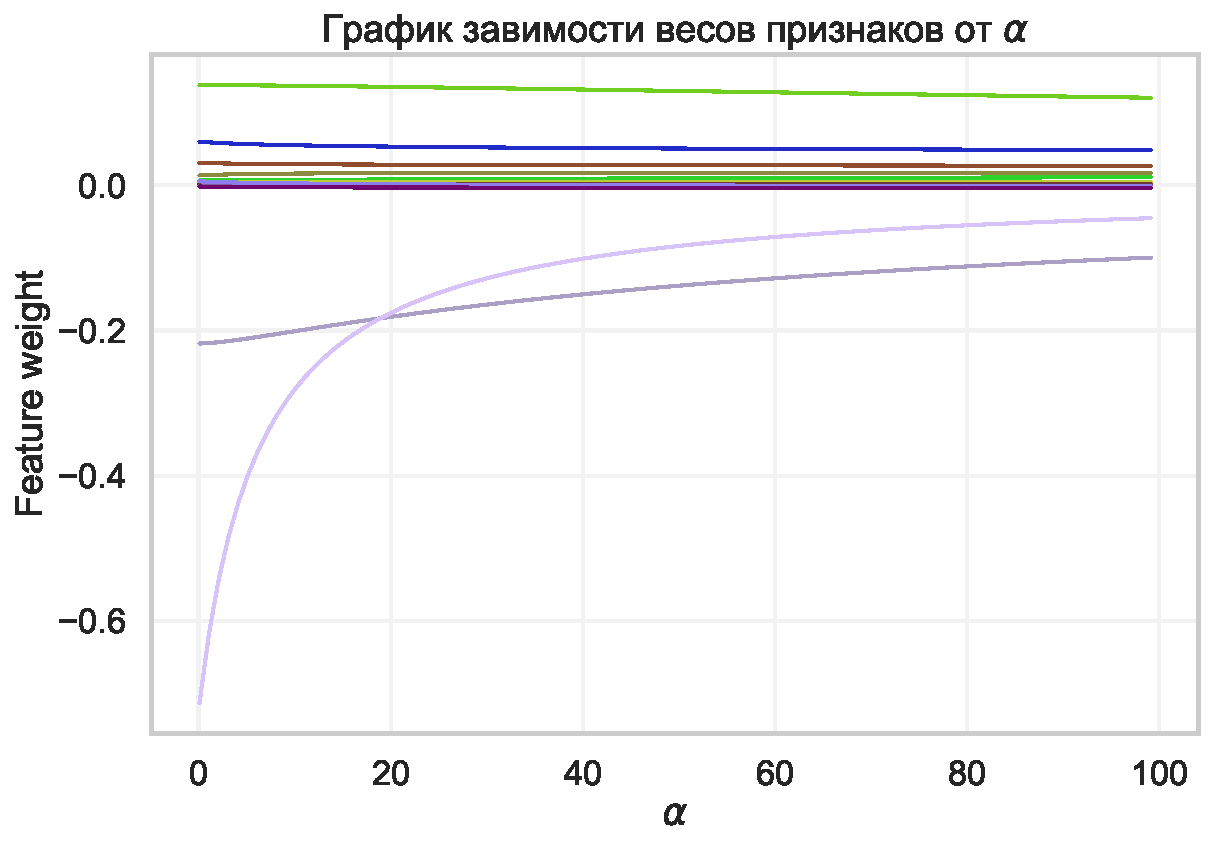
\includegraphics[width=\textwidth]{feature_plot_1.pdf}
            \end{subfigure} 
        \end{figure}
    \end{frame}

    \begin{frame}{Изменение параметра $\alpha$ при стандартизации}
        \begin{figure}
            \centering
            \begin{subfigure}[b]{0.475\textwidth}
                \centering
                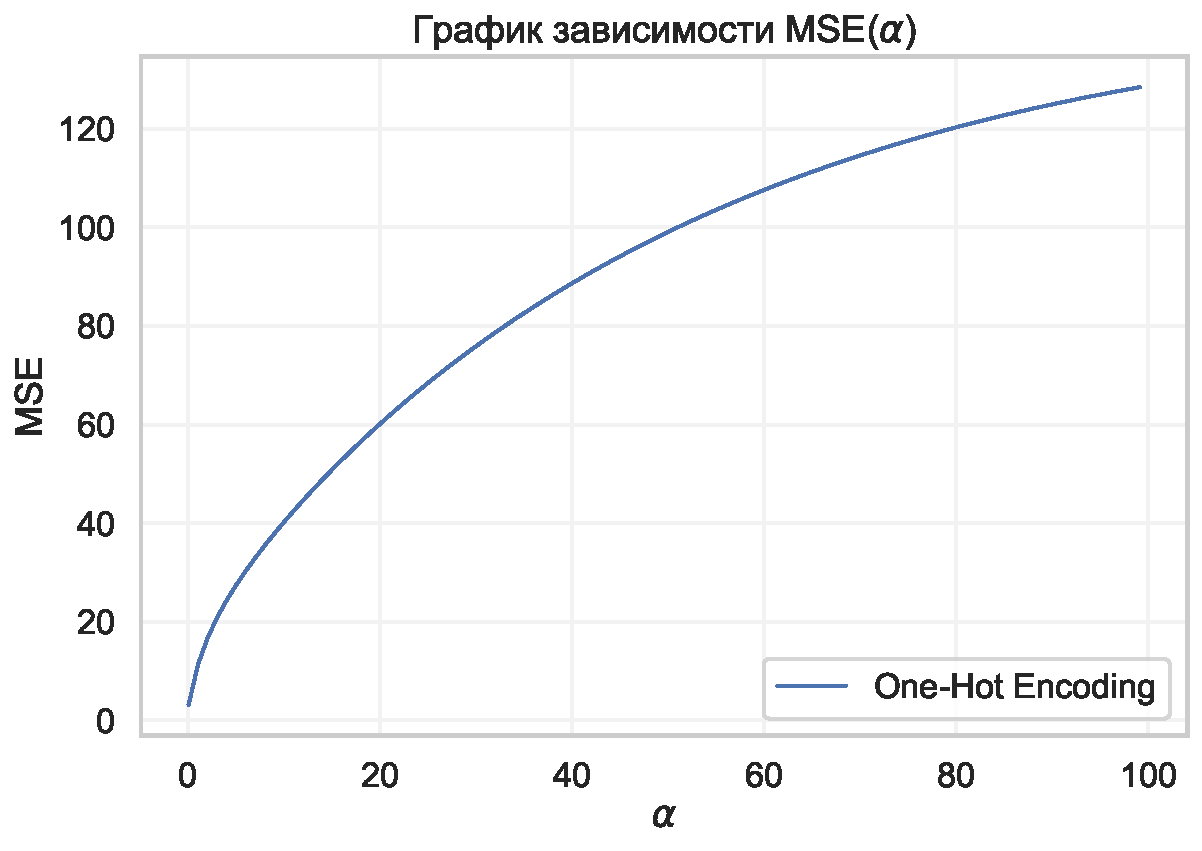
\includegraphics[width=\textwidth]{MSE_plot_oh_scaled_1.pdf}
            \end{subfigure}
            \hfill
            \begin{subfigure}[b]{0.475\textwidth}  
                \centering 
                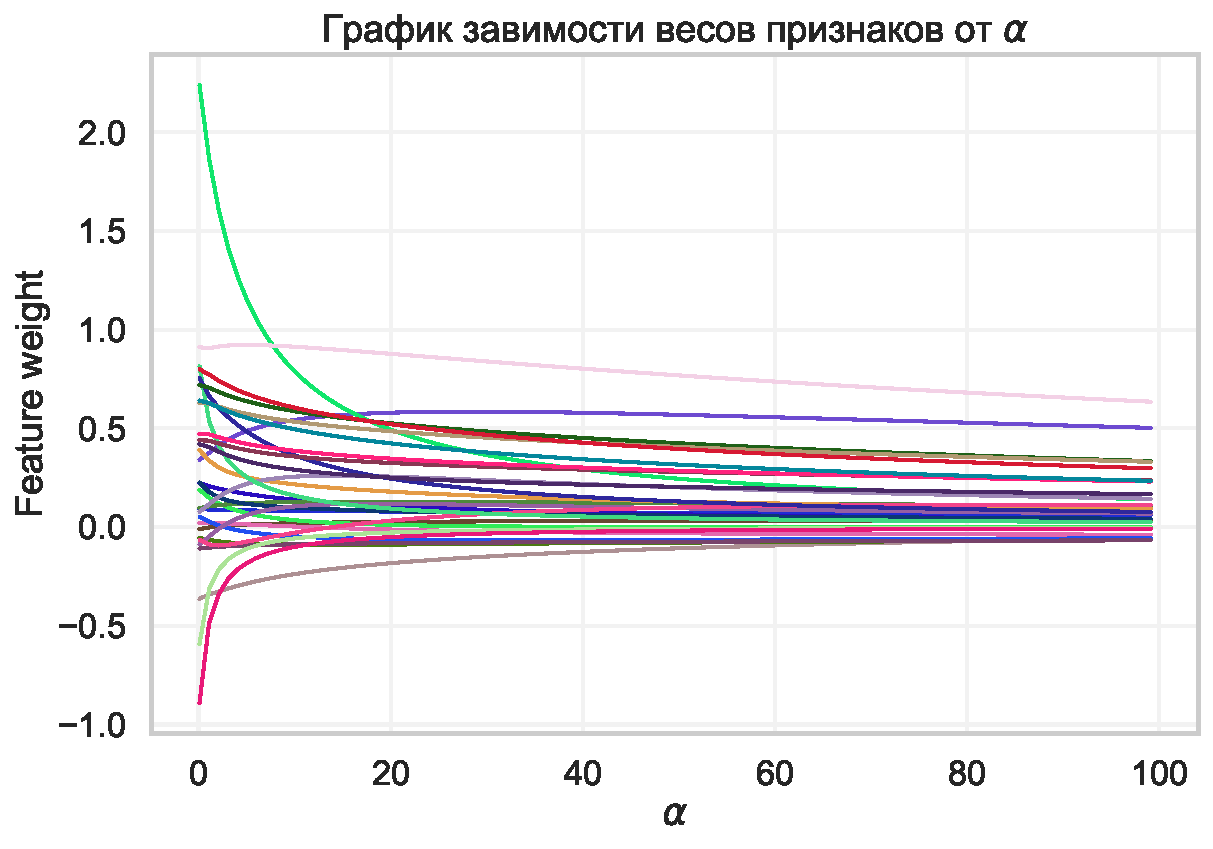
\includegraphics[width=\textwidth]{feature_plot_oh_scaled_1.pdf}
            \end{subfigure}
            \begin{subfigure}[b]{0.475\textwidth}   
                \centering 
                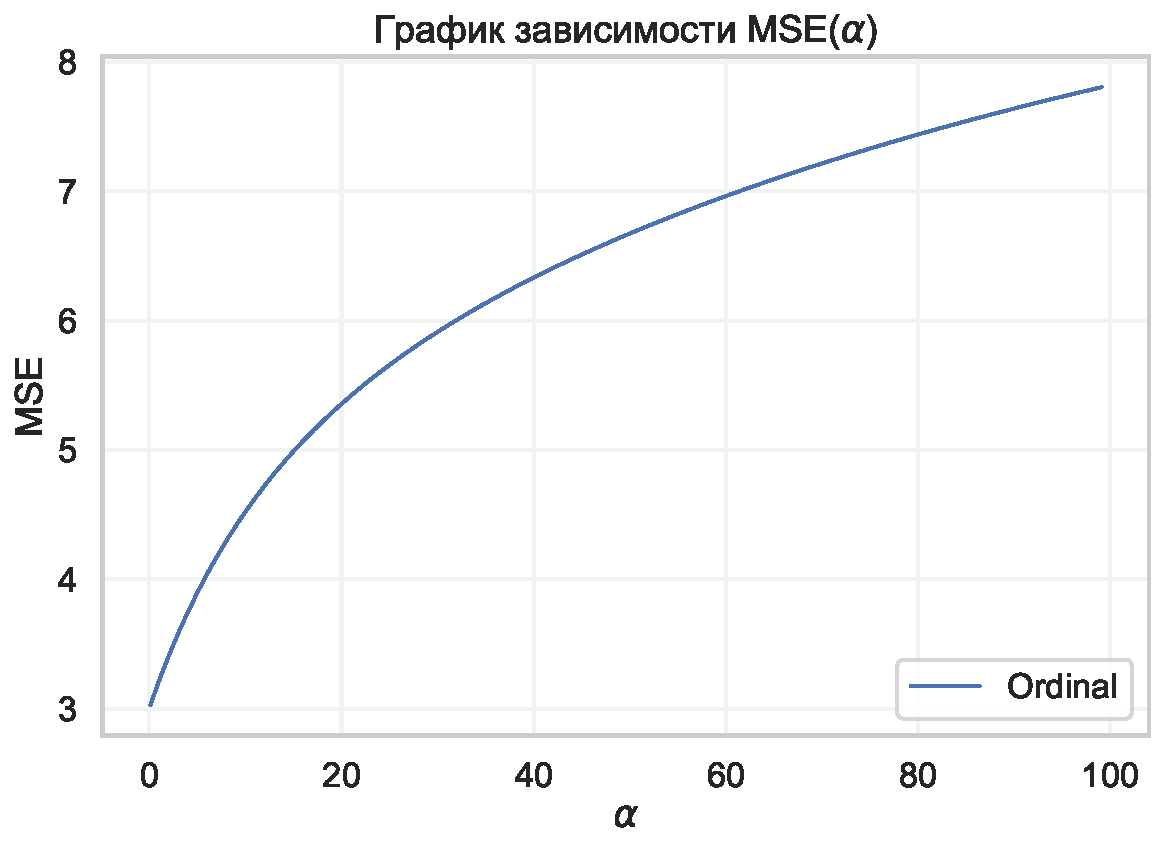
\includegraphics[width=\textwidth]{MSE_plot_scaled_1.pdf}
            \end{subfigure}
            \hfill
            \begin{subfigure}[b]{0.475\textwidth}   
                \centering 
                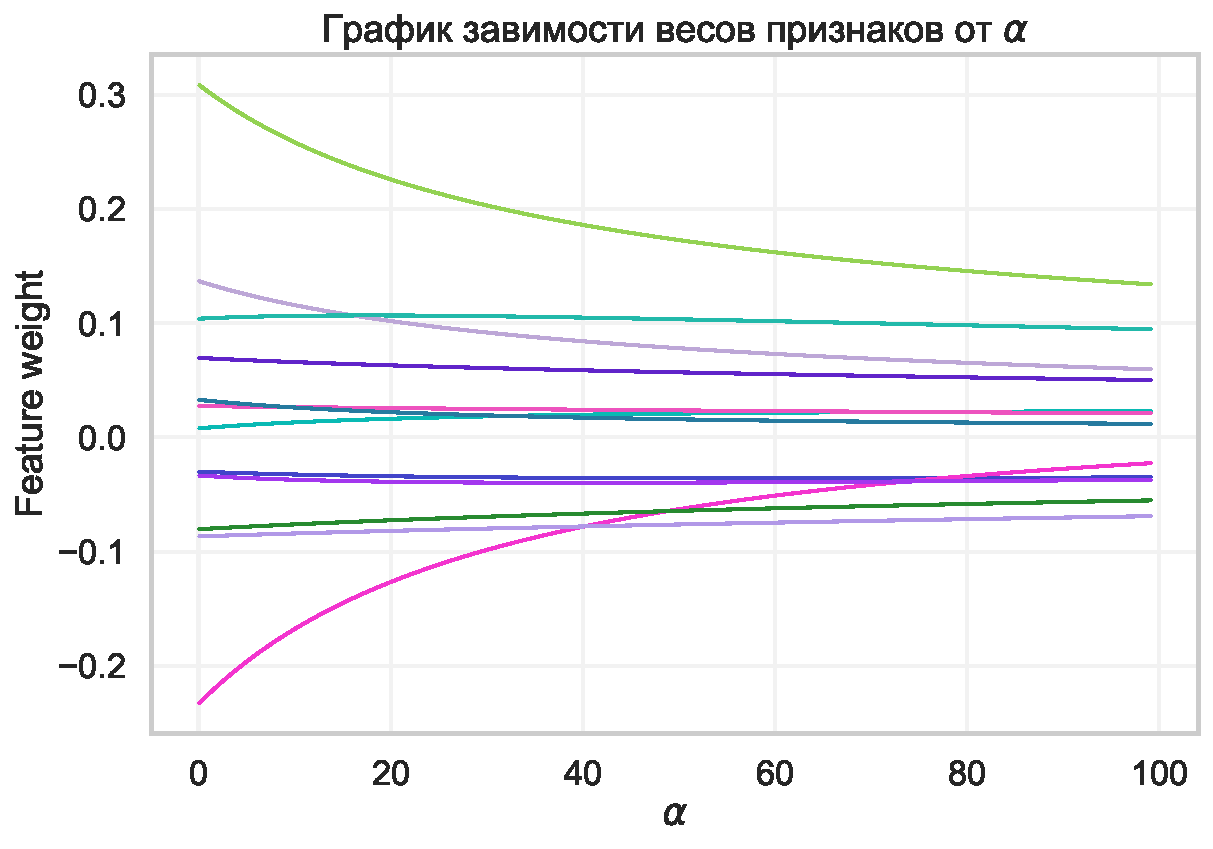
\includegraphics[width=\textwidth]{feature_plot_scaled_1.pdf}
            \end{subfigure} 
        \end{figure}
    \end{frame}

    \begin{frame}{Сравнение результатов}
        \begin{table}[h!]
            \centering
            \begin{tabular}{|c|c|c|}
                \hline
                \diagbox{Стандартизация}{Преобразование} & До       & После  \\ \hline
                - & 616,50                 & 1,82                    \\ \hline
                + & 624,78                 & 1,89                    \\ \hline
            \end{tabular}
            \caption{Лучшее значение MSE на кросс-валидации}
        \end{table}

        Стоит отметить, что после преобразования ответами являются $\ln(1 + area)$.

    \end{frame}

    \begin{frame}{Наиболее значимые признаки}
        Значимость признаков при решении задачи лучше всего оценивается на данных
        после преобразования. Таковыми являются:
        \begin{itemize}
            \item month~--- месяц года
            \item wind~--- скорость ветра
            \item rain~--- количество осадков
            \item DC и DMC~--- индексы засухи и влажности почвы
        \end{itemize}
    \end{frame}

\end{document}